\documentclass[../ana1.tex]{subfiles}
\onlyinsubfile{\sectionNumbering} %Use numbering relative to sections and not subsection

\begin{document}
\setcounter{section}{7}

\section{Monotone Konvergenz}
\begin{defi}
	Eine Folge \({(a_n)}_n\) heißt \\
	monoton wachsend, falls \(a_n\leq a_{n+1} \quad \forall n\in\N \).\\
	monoton fallend, falls \(a_{n+1} \leq a_n \quad\forall n\in\N \).\\
	Ähnlich: monoton wachsend (fallend) für fast alle \(n\in\N \), falls \( K\in\N \) existiert mit \( a_n\leq a_{n+1} \quad \forall n\geq K \) (bzw. \(a_{n+1}\leq a_n \quad \forall n\geq K \)).\\
	Ist \\
	\( a_n<a_{n+1} \quad \forall n\in\N \), so heißt \(a_n\) streng monoton wachsend.\\
	\( a_{n+1}<a_n \quad \forall n\in\N \), so heißt \(a_n\) streng monoton fallend.
\end{defi}
\begin{satz}[Monotone Konvergenz]
	Jede monoton wachsende, nach oben beschränkte Folge ist konvergent. Jede monoton fallende, nach unten beschränkte Folge ist konvergent.
\end{satz}
\begin{bew}
	\({(a_n)}_{n\in\N}, a_{n+1} \geq a_n \quad \forall n\in\N \) (oder \( \forall n\geq K \in\N \))\\
	und \( \exists C\in\R: a_n \leq C \quad \forall n\in\N \) (oder \( \forall n\geq K \in\N \))\\
	\[ B:= \{a_n, n\in\N \} \subset \R, b\neq \emptyset \text{ und } B\leq C. \]
	\(\overset{\text{Vollst.axiom}}{\Rightarrow} L := \sup B\) die kleinste obere Schranke für \(B\).\\
	\(\Rightarrow a_n \leq L \quad \forall n\in\N \).\\
	Und: \(L\) kleinste ob. Schranke \( \Rightarrow \forall \varepsilon>0: L-\varepsilon \) keine obere Schranke für \(B\).\\
	\[ \Rightarrow \exists K \in\N: L-\varepsilon < a_K \leq a_{K+1} \leq a_{K+2} \leq \cdots \leq a_n \quad \forall n\geq K. \]
	\[ \forall n\geq K: L-\varepsilon < a_n \leq L < L + \varepsilon \Leftrightarrow a_n \in (L-\varepsilon, L + \varepsilon) \]
	\( \Leftrightarrow {(a_n)}_n \) konvergiert gegen \(L\).\\
	Ist \(a_{n+1} \leq a_n, a_n\geq C \quad \forall n\in\N \), so betrachte \(b_n := -a_n \leq -C \) und \(b_{n+1} \geq b_n\). Dann ersten Fall anwenden!
\end{bew}
\begin{bsp}[1]
	\(x_0 > 0, \quad x_{n+1} := \frac{1}{2} \left( x_n + \frac{a}{x_n} \right) \) konvergent gegen \(\sqrt{a}, a>0 \).\\
	Ang.: \( \limes{n} x_n = l \) existiert, dann auch \( \limes{n} x_{n+1} = l, l>0 \)
	\[ \overset{\text{Grenzwertsätze}}{\Longrightarrow} l = \limes{n} x_{n+1} = \limes{n} \left( \frac{1}{2} \left(x_n + \frac{a}{x_n} \right) \right) = \frac{1}{2} \left( l + \frac{a}{l} \right) \Rightarrow l^2 = a, l = \sqrt{a}. \]
\end{bsp}
\begin{bsp}[2]
	\(f_n := {\left( 1 + \frac{1}{n} \right)}^n \) Grenzwert \( \limes{n} f_n = \limes{n} {\left( 1 + \frac{1}{n} \right)}^n \) existiert \( =: e \).\\
	Beh. 1: \( f_n\) ist nach oben beschränkt.\\
	Beh. 2: \( f_n\) ist monoton wachsend.
\end{bsp}
%22.11.2018
\begin{bew}
	Beh. 1:
	\begin{align*}
		f_n = {(1+\frac{1}{n})}^n  &= \sum_{k=0}^{n} \binom{n}{k} {\left( \frac{1}{n} \right)}^k\\
		&= \sum_{k=0}^{n} \underbrace{\frac{n!}{k!(n-k)!}}_{=\frac{n(n-1)\ldots (n-k+1)}{k!}} \\
		&= \sum_{k=0}^{n} \frac{1}{k!} \frac{n}{n} \underbrace{\frac{n-1}{n}}_{<1} \underbrace{\frac{n-k+1}{n}}_{<1}\\
		&\leq \sum_{k=0}^{n} \frac{1}{k!} =: e_n, \quad f_n \leq e_n \forall n\in\N \\
		e_{n+1} = e_n + \frac{1}{(n+1)!} > 1_n.
	\end{align*}
	Beachte: \( k! = k(k-1)(k-2)\ldots3\cdot2\cdot1 \qquad k\geq 2 \) \\
	\( \geq 3\cdot3\ldots3\cdot2\cdot1 = 3^{k-2}\cdot2 (*) \) \\
	Also ist \(n\geq3\).
	\begin{align*}
		e_n = \sum_{k=0}^{n} \frac{1}{k!} = 1+1 + \sum_{k=2}^{n} \frac{1}{k!} \overset{(*)}{\leq} 2 + \sum_{k=2}^{n} \frac{1}{2 \cdot 3^{k-2}}\\
		= 2 + \frac{1}{2} \underbrace{\sum_{l=0}^{n-2} {(\frac{1}{3})}^l}_{=1 - {(\frac{1}{3})}^{n-1}}\\
		\leq 2 + \frac{1}{2} \cdot \frac{3}{2} = 2 + \frac{3}{4} = 2,75.\\
		\Rightarrow e_n \leq 2,75 \forall n\geq 2.
	\end{align*}
	\(\Rightarrow {(e_n)}_n \) ist nach oben beschränkt.\\
	\( \overset{\text{Mon.\ Konv.}}{\Rightarrow} \limes{n} e_n \) existiert \(\leq 2,75\).\\
	Auch \( f_n\leq e_n\leq 2,75 \quad \forall n\geq 2 \).\\
	\( \Rightarrow {(f_n)}_n \) ist auch oben beschränkt.
	Beh. 2:\\
	\begin{align*}
		\frac{f_n}{f_{n-1}} &= \frac{{(1+\frac{1}{n})}^n}{{(1+\frac{1}{n})}^{n-1}} \qquad n\geq 2\\
		&= \frac{{(\frac{n+1}{n})}^n}{{(\frac{n}{n-1})}^{n-1}} = \frac{n}{n-1} \frac{{(\frac{n+1}{n})}^n}{{(\frac{n}{n-1})}^{n}} \frac{n}{n-1} {\left( \frac{\overbrace{(n+1)(n-1)}^{n^2-1}}{n^2} \right)}^n\\
		&= \frac{n}{n-1} {\left( \frac{n^2-1}{n^2} \right)}^n = \frac{n}{n-1} \underbrace{{\left( 1-\frac{1}{n^2} \right)}^n}_{\geq 1-n \frac{1}{n^2} \text{ (Bern. Ungl.)}}\\
		&\geq \frac{n}{n-1} (1-n \frac{1}{n^2}) = \frac{n}{n-1} (1-\frac{1}{n}) = 1 \Rightarrow f_n \geq f_{n-1} \forall n\geq 2.
	\end{align*}
	\( \Rightarrow \limes{n} f_n \) existiert!
\end{bew}
\begin{defi}[Eulersche Zahl]
	\( e:= \limes{n} {(1+\frac{1}{n})}^n \) (\(\leq 2,75\))
\end{defi}
\begin{bem}
	\begin{enumerate}
		\item Es gilt auch \( \limes{n} {(1+\frac{x}{n})}^n \) exist. \( \forall x\in\R \) (H.A.)
		\item Alternative Darstellung für \(e\):\\
		Hatten gesehen: \(f_n \leq e_n = \sum_{k=0}^{n} \frac{1}{k!} \quad \forall n \) \\
		\(e_n \leq 2,75, e_{n+1} > e_n \) \\
		\( \Rightarrow \) es existiert \( \limes{n} e_n = \limes{n} \sum_{k=0}^{n} \frac{1}{k!} =: \sum_{k=0}^{\infty} \frac{1}{k!} \) und somit auch \(e = \limes{n} f_n\leq \limes{n} e_n = \sum_{k=0}^{\infty} \frac{1}{k!} \).
	\end{enumerate}
	Beobachtung: 
	\[ f_n = {\left(1+\frac{1}{n}\right)}^n = \sum_{k=0}^{n} \frac{1}{k!} \underbrace{\frac{n}{n}\frac{(n-1)}{n} \ldots\frac{n-k+1}{n}}_{\geq 0} , \quad {\left(1+\frac{1}{n}\right)}^n = \sum_{k=0}^{n} \binom{n}{k} \frac{1}{n^k}. \]
	Nehme \(m\in\N \) fest.
	\[ n\geq m \geq \sum_{k=0}^{m} \frac{1}{k!} 1 \underbrace{\frac{n-1}{n}}_{\overset{n\rightarrow\infty}{\rightarrow} 1} \ldots \underbrace{\frac{n-k+1}{n}}_{\overset{n\rightarrow\infty}{\rightarrow} 1} \]
	Grenzwertsätze \(\Rightarrow \sum_{k=0}^{m} \frac{1}{k!} \) für \(n\rightarrow\infty \).
	\( \Rightarrow \) Für jedes \(m\in\N \) ist
	\[e_m \leq \limes{n} f_n = e \]
	Auch, \(e_m = \sum_{k=0}^{m} \frac{1}{k!} \) hat den Grenzwert \(m\rightarrow\infty \)!
	\[ \overset{\text{Satz 7.1.9.}}{\lim\limits{m\rightarrow\infty}} e_m \leq e. \]
	\[\Rightarrow e = \lim\limits_{m\rightarrow\infty} \sum_{k=0}^{m} \frac{1}{k!} =: \sum_{k=0}^{\infty} \frac{1}{k!} \]
\end{bem}
\begin{satz} 
	\(e\) ist irrational!
\end{satz}
\begin{bew}
	\(e_n = \sum_{k=0}^{n} \frac{1}{k!} \) approximiert \(e\) extrem gut\\
	\[ 0< e-e_n = \sum_{k=0}^{\infty} \frac{1}{k!} - \sum_{k=0}^{n} \frac{1}{k!} = \sum_{k=n+1}^{\infty} \frac{1}{k!}. \]
	\[e-e_n = \limes{n}\left( \sum_{k=0}^{m} \frac{1}{k!} - \sum_{k=0}^{n} \frac{1}{k!} \right) = \limes{m} \left(\sum_{k=n+1}^{n} \frac{1}{k!} \right) \]
	\begin{align*}
	 	(*)\quad k \geq n+1\\
		k! &= k(k-1)\dots 3\cdot 2\cdot 1\\
		&=\underbrace{k(k-1)\dots(n+2)}_{\geq 2^{k-n}}\underbrace{(n+1)n\dots 2\cdot 1}_{=(n+1)!} \geq (n+1)!\\
		&\geq 2^{k-n}(n+1)!
	\end{align*}
	\begin{align*}
		m>n: &\sum_{k=n+1}^{m} \frac{1}{k!}\\
		&\overset{(*)}{\leq} \sum_{k=n+1}^{m} \frac{1}{(n+1)!} {\left(\frac{1}{2}\right)}^{k-(n+1)}\\
		&\leq \frac{1}{(n+1)!} \sum_{k=n+1}^{m} {\left(\frac{1}{2}\right)}^{k-(n+1)}\\
		&= \frac{1}{(n+1)!} \sum_{l=0}^{m-(n+1)} {(\frac{1}{2})}^l = \frac{1}{(n+1)!} \frac{1-{(\frac{1}{2})}^{m-(n-1)}}{1-\frac{1}{2}}\\
		&\leq \frac{1}{(n+1)!} \frac{1}{1-\frac{1}{2}} = \frac{2}{(n+1)!}\\
		&\Rightarrow 0 < e - e_n \leq \frac{2}{(n+1)!} (*) \qquad\forall n\geq 2.
	\end{align*}
	Wäre \(e\) rational, \(\Rightarrow p\in\N,q\in\N:e=\frac{p}{q} \)
	\[ \Rightarrow n! e = n! \frac{p}{q} \in\N \forall n\geq q \]
	Auch: \( n! e_n = n! \sum_{k=0}^{n} \frac{1}{k!} \in\N \) \\
	\( \Rightarrow n!(e-e_n) \in\N_0 \qquad \forall n \), die groß genug sind
	\[ \overset{(*)}{\Rightarrow} 0<n!(e-e_n) \leq \frac{n!2}{(n+1)!} = \frac{2}{n+1} < 1 \quad \forall n\geq 3 \]
	\Lightning{} also ist \(e\) irrational!
\end{bew}
\textbf{Anwendungen:}
\begin{satz}[Invervallschachtelungsprinzip]
	Seien \( a_n\leq b_n, I_n := [a_n,b_n] \) abgeschlossene Intervalle und \[I_{n+1} \subset I_n \quad \forall n\in\N \]
	sowie \( |I_n| := b_n - a_n \overset{n\rightarrow\infty}{\rightarrow} 0 \).\\
	Dann besteht \(\bigcap_{n\in\N} I_n\) aus genau einem Punkt!\\
	Bild: 
	\begin{center}
		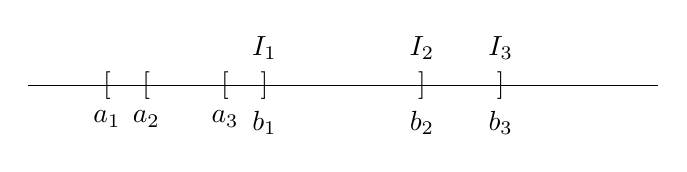
\begin{tikzpicture}
			\draw (0,0) -- (8,0);
			\draw (1,0) node {\([\)} node[below=2mm] {\(a_1\)};
			\draw (1.5,0) node {\([\)} node[below=2mm] {\(a_2\)};
			\draw (2.5,0) node {\([\)} node[below=2mm] {\(a_3\)};
			\draw (3,0) node {\(]\)} node[below=2mm] {\(b_1\)} node[above=2mm] {\(I_1\)};
			\draw (5,0) node {\(]\)} node[below=2mm] {\(b_2\)} node[above=2mm] {\(I_2\)};
			\draw (6,0) node {\(]\)} node[below=2mm] {\(b_3\)} node[above=2mm] {\(I_3\)};
		\end{tikzpicture}
	\end{center}
\end{satz}
\begin{bew}
	\begin{enumerate}
		\item \( \bigcap_{n\in\N} I_n \) besteht aus höchstens einem Punkt in \(\R \).\\
		Ang. \( \exists a, a^2 \in \bigcap_{n\in\N} I_n \quad a\neq a^2 \) (o.B.d.A. \(\tilde{a}>a\)).\\
		\[I_{n+1} \subset I_n \quad\forall n \Rightarrow I_n \subset I_{n-1} \subset \ldots\subset I_m \quad \forall n>m.\]
		\[ \Rightarrow \bigcap_{n\in\N} I_n = \{ x\in\R| x\in I_n \forall n\in\N \} \subset \{ x\in\R|x\in I_k \quad \forall 1\leq k \leq m \} = \bigcap_{k=1}^m I_k = I_m \]
		\[ \Rightarrow \{ a,\tilde{a} \} \subset I_m \quad\forall m\in\N. \]
		\[a,\tilde{a} \in I_m = [a_m,b_m]. \]
		\begin{center}
			\begin{tikzpicture}
				\draw (0,0) -- (5,0);
				\draw (1,0) node {\([\)} node[below=2mm] {\(a_m\)};
				\draw (4,0) node {\(]\)} node[below=2mm] {\(b_m\)};
				\draw (2,-0.1) -- (2,0.1) (3,-0.1) -- (3,0.1);
				\draw (2,0) node[below] {\(a\)} (3,0) node[below] {\(\tilde{a}\)};
			\end{tikzpicture}
		\end{center}
		\[\Rightarrow 0<\tilde{a}-a \leq b_m - a_m = |I_m| \rightarrow 0 \quad m\rightarrow\infty \]
		\Lightning{} für \(m\) groß \(\bigcap_{n\in\N} I_n\) hat höchstens ein Element!
		\item \( \bigcap_{n\in\N} I_n \neq \emptyset \qquad I_n = [a_n,b_n] \) \\
		\[I_{n+1} \subset I_n \Leftrightarrow a_{n+1} \geq a_n \wedge b_{n+1} \leq b_n \quad \forall n. \]
		Auch: \( a_n \leq b_n \leq b_{n-1} \leq \cdots\leq b_1 \)
		\( \Rightarrow \) Folge \({(a_n)}_n\) ist nach oben beschränkte monoton wachsende Folge.\\
		\( \overset{\text{Mon.Konv.}}{\Rightarrow} a:= \limes{n} a_n \) existiert und \(a\geq a_n \quad \forall n \).\\
		Sei \(n\geq m\):
		\[a-n\leq b_n\leq\cdots\leq b_m \Rightarrow a = \limes{n} a_n \leq b_m \]
		\[\Rightarrow a_m\leq a_{n-1}\leq a_n\leq a\leq b_m. \]
		\( \Rightarrow a\in I_m\) für jedes \(m\in\N \) \\
		\[  \Rightarrow \{a\}\subset \bigcap_{m\in\N} I_m \]
		\[ \text{d.\ h.\ } \bigcap_{m\in\N} I_m \neq \emptyset \]
	\end{enumerate}
\end{bew}
\begin{satz}[\(k\)-adische Darstellung reeller Zahlen]
	\(k\in\N, k\geq Z\) und \(x\in\R \). Dann gibt es \(z_0\in \Z \) und \(l_j \in \{0,1,\ldots,k-1\} \) derart, dass \(x = z_0 + \limes{n} \sum_{j=1}^{n} l_j k^{-j} = z_0 + \sum_{j=1}^{\infty} l_j k^{-j} \).\\
	\(Z_0 := \lfloor x \rfloor := \min(p\in\Z, p>x) -1 = \max(q\in\Z, q\leq x). \) \\
	\( 0\leq x-\lfloor c\rfloor <1. \) \\
	\(\Rightarrow \) o.\ B.\ d.\ A.\ sei \(0\leq x<1\).
	\begin{center}
		\begin{tikzpicture}
			\draw (0,0) -- (8,0);
			\foreach \x in {0,...,8}
			\draw (\x, 0.1) -- (\x, -0.1);
			\draw (3,0) node[above = 1mm, font=\fontsize{6}{0}] {\(l_1 = 3\)};
			\draw (4,0) node[above = 1mm, font=\fontsize{6}{0}] {\(l_1 + 1 = 4\)};
			\draw (0,0) node[below = 2mm] {\(0\)};
			\draw (8,0) node[below = 2mm] {\(1\)};
			\foreach \x in {1,...,9}
			\draw (3.\x, 0.05) -- (3.\x, -0.05);
			\draw (3.5,0) node[below = 2mm] {\(x\)};
		\end{tikzpicture}
	\end{center}
	iteriere diesen Prozess.
	\(\rightarrow \) kriegen \(l_j \in \{0,1,2,\ldots,k-1 \} \) und \(\sum_{j=1}^{n} l_j k^{-j} \leq x < \sum_{j=1}^{n-1} l_j k^{-j + \frac{l_n + 1}{k^n}} \quad (*)\) \\
	\[ \overset{(*)}{\Rightarrow} x = \limes{n} \sum_{j=1}^{n} l_j k^{-j}. \]
\end{satz}
%27.11.2018
\begin{bsp}
	\( p := \lfloor x \rfloor := \max (z\in\Z:z\leq x) \Rightarrow p\leq x < p+1 \Rightarrow \tilde{x} := x - p \in [0,1) \). Also reicht es, \(x\in[0,1)\) zu betrachten!\\
	Bild: \(k=8\) \\
	\begin{center}
		\begin{tikzpicture}
		\draw (0,0) -- (8,0);
		\foreach \x in {1,...,7}
		\draw (\x, 0.1) -- (\x, -0.1);
		\draw (3,0) node[above = 1mm, font=\fontsize{6}{0}] {\(l_1 = 3\)} node[below = 1mm] {\(\frac{3}{8}\)};
		\draw (4,0) node[above = 1mm, font=\fontsize{6}{0}] {\(l_1 + 1 = 4\)} node[below = 1mm] {\(\frac{4}{8}\)};
		\draw (0,0) node {\([\)} node[below = 2mm] {\(0\)};
		\draw (8,0) node {\()\)} node[below = 2mm] {\(1\)};
		\end{tikzpicture}
	\end{center}
	\(l_1 = \lfloor kx \rfloor \)
	\[ \frac{l_1}{k} \leq x < \frac{l_1 + 1}{k} \Rightarrow 0 \leq x - \frac{l_1}{k} < \frac{1}{k} \]
	\[ \Rightarrow 0 \leq k\left( x - \frac{l_1}{k} \right) < 1 \Leftrightarrow 0 \leq k^2 [x-\frac{l_1}{k}] < k. \]
	\[ l_2 := \lfloor k^2\left( x - \frac{l_1}{k} \right) \rfloor \overset{\text{wie vorher}}{\Rightarrow} \frac{l_2}{k} \leq k(x-\frac{l_1}{k}) < \frac{1}{k} \]
	\[ \Rightarrow l_1/k + l_2/k^2 \leq x < l_1/k + \frac{l_2 + 1}{k^2} \]
	induktiv weitermachen. Geg. \( l_1, l_2, \ldots, l_n \in \{ 0,1,2,\ldots,k-1 \} \). 
	\[ \text{mit } l_1/k + l_2/k^2 + \cdots + l_n/k^n \leq x < l_1 /k + l_2/k^2 + l_{n-1}/k^{n-1} + \frac{l_n + 1}{k^n} \]
	\[ \Rightarrow 0\leq x - \sum_{j=1}^{n} \frac{l_j}{k^j} < \frac{1}{k^n} \]
	\[ \text{oder } k^{n+1} [x-\sum_{j=1}^{n} \frac{l_j}{k^j} ] < k\in\N \]
	\[ \text{definiere } l_{n+1} := \lfloor k^{n+1} (x-\sum_{j=1}^{n} \frac{l_j}{k^j} ) \rfloor  \]
	\[ \text{kriegen } a_n := \sum_{j-1}^{n} \frac{l_j}{k^j} \leq x < \sum_{j=1}^{n} l_j/k^j + 1/k^n =: b_n \]
	\[ \Rightarrow a_n \leq x < b_n \]
	\[ \text{und } b_n - a_n = 1/k^n \rightarrow 0, n\rightarrow\infty. \]
	Entweder: \(I_n := [a_n,b_n] \) sind geschachtelt \(I_{n+1} \subset I_n \)
	Lange \(I_n - |I_n| = b_n - a_n \rightarrow 0. \)
	Intervallschachtelungsprinzip \(\Rightarrow \{x\} = \bigcap_{n\in\N} I_n \)
	\( \Rightarrow x= \limes{n} a_n = \limes{n} \sum_{j=1}^{n} l_j/k^j \).\\
	Alternative:\\
	\begin{align*}
		a_{n+1} &\geq a_n\\
		a_n &\leq b_n = \sum_{j=1}^{n} \frac{l_j}{k^j} + \frac{1}{k^n}\\
		&\leq \sum_{j=1}^{n} \frac{k-1}{k^j} + \frac{1}{k^n}\\
		&= (k-1)\underbrace{ \sum_{j=1}^{n} {( \frac{1}{k})}^j + \frac{1}{k^n} }_{= \frac{1}{k} \sum_{j=0}^{n-1} {(\frac{1}{k})}^j = \frac{1}{k} \frac{1-{(\frac{1}{k})}^n}{1-\frac{1}{k}} }\\
		&=\frac{k-1}{k}-\frac{1-{(\frac{1}{k})}^n}{1-\frac{1}{k}} + \frac{1}{k^n}\\
		&= 1- {\left(\frac{1}{k}\right)}^n + \frac{1}{k^n} = 1.\\
		\overset{\text{Mon. Konv.}}{\Rightarrow} a &= \limes{n} a_n \text{ existiert.}\\
	\end{align*}
	Beachte: \(0 \leq x-a_n < \frac{1}{k^n} \rightarrow\overset{n \rightarrow \infty}{\rightarrow} 0\) \\	 
	\begin{align*}
		a_n \leq x < a_n + \frac{1}{k^n} \Rightarrow\overset{\text{Sandwich}}{\Rightarrow}
		a &= \limes{n} a_n \leq x \leq \limes{n} a_n + \limes{n} \frac{1}{k^n}\\
		&= a + 0 = a\\
		&\Rightarrow a \leq x \leq a \Rightarrow a = x
	\end{align*}
\end{bsp}
\begin{bsp}
	\(k\)-adische Darstellung\\
	\(k = 10\) \\
	Behauptung: \(0\text{,}\overline{9} = 1\)
	\begin{align*}
		0\text{,}\overline{9} &= \limes{n} \sum_{j=1}^{n} \frac{9}{10^j}\\
		&=\limes{n} \frac{9}{10}\cdot \sum_{j=0}^{n-1}{\left(\frac{1}{10}\right)}^j\\
		&=\frac{9}{10}\cdot\frac{10}{9} = 1
	\end{align*}
\end{bsp}
\begin{kor}
	Die reellen Zahlen sind überabzählbar!
\end{kor}
\begin{bew}
	Es reicht zu zeigen \( [0,1) \) ist überabzählbar. Es reicht, eine Teilmenge von \(A \subset [0,1) \) anzugeben, die nicht abzählbar ist.\\
	nehmen: \(k=3\)
	\[ A:= \{ x\in[0,1) : \exists l_j \in \{0,1 \}: x = \sum_{j=1}^{\infty} \frac{l_j}{3^j} = \limes{n} \sum_{j=1}^{n}\frac{l_j}{3^j} \}. \]
	\(A\) hat die gleiche Mächtigkeit wie die Menge der \( \{0,1\} \)-wertigen Folgen. Hat dieselbe Mächtigkeit wie \(\mathcal{P}(\N)\). Diese ist überabzählbar.
\end{bew}

\end{document}